% !TeX spellcheck = en_GB
\subsection{Simulation based optimization}

Simulation based optimization is often used in combination with repairable
systems.

\subsubsection{Repairable systems}
Consider highly complex systems such as aircrafts, oil drilling and nuclear
power plants. These systems contain thousands of critical, expensive
components. To avoid enormous costs that result from system failures,
such systems keep an inventory of spare parts which are flown directly to
the interruption site (for instance to the oil drilling platforms). The defective
parts can be repaired at an on-site repair shop.

\paragraph{Assumptions}

\begin{itemize}
	\tightlist
	\item Each component failure makes the system go down.
	\item The technical systems and its spare parts are produced in a single
	batch. Reordering is not possible/allowed.
	\item The repair center can be modeled as a single server queue, i.e. only
	one item can be repaired at the same time.
	\item Transportation times between oil platform, stocking location, and repair
	center can be ignored.
\end{itemize}

\paragraph{Tasks}
\begin{description}
	\item[Objective] Minimize the sum of annual downtime costs, annual amortized
	purchasing costs and annual inventory holding costs.
	\item[Strategic decision] How many items do we purchase (produce) at time
	$t = 0$?
	\item[Operational decisions] How to prioritize the repair jobs at the repair
	center?
\end{description}

\subsubsection{Flow Diagram}
\begin{figure}[H]
	\centering
	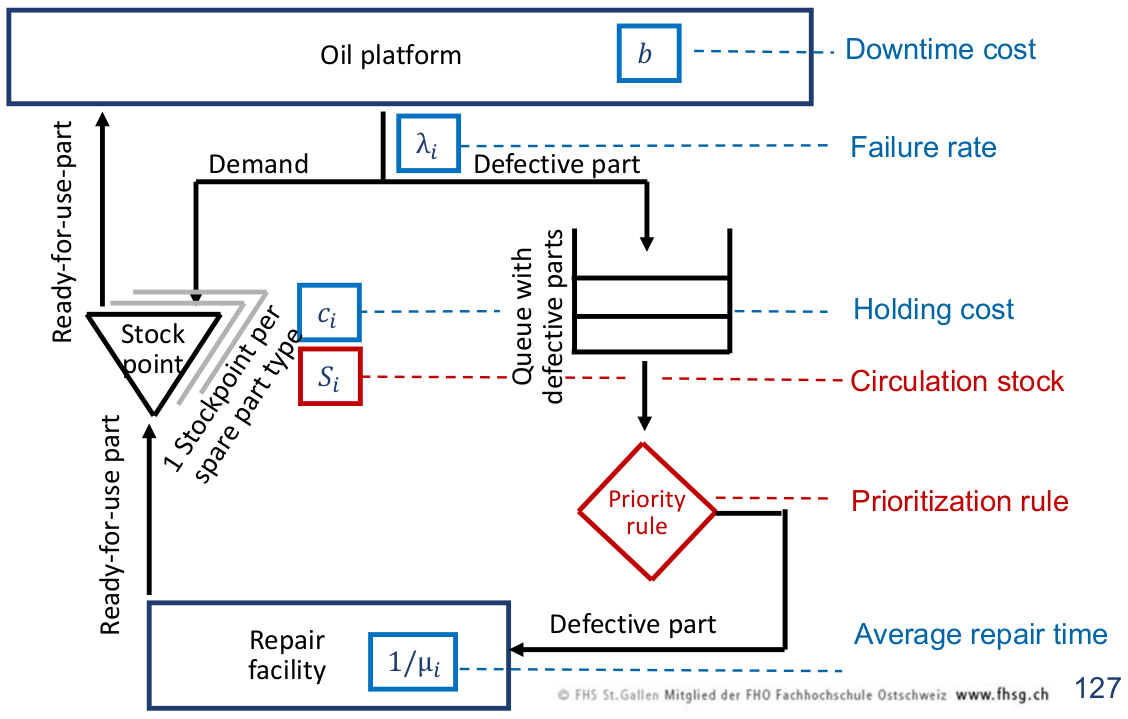
\includegraphics[width=0.8\textwidth]{figures/RepairableSystemDES.png}
	\caption{Flow diagram of a repairable system}
\end{figure}

\subsubsection{Solution path}

\begin{enumerate}
	\tightlist
	\item Develop a simulation model, that calculates for given circulation
	stocks and a given prioritization rule, the average annual total cost
	as well as the evolution of spare part stock over time.
	\item Develop via experimenting with the simulator, a reasonable
	prioritization rule for jobs at the repair facility.
	\item Develop a simulation-based optimization model.
\end{enumerate}

\subsubsection{Analysis}

The simulation results in an event table like the one in
\autoref{fig:SimOptimiz-ProcessLogic}.
\begin{figure}[H]
	\centering
	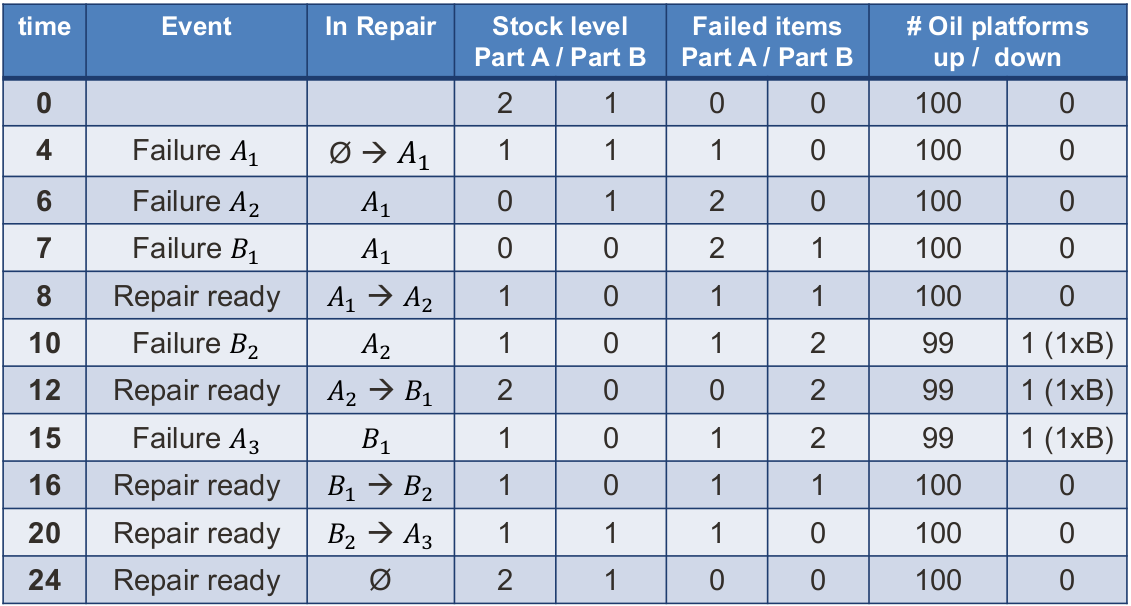
\includegraphics[width=0.8\textwidth]{figures/SimOptimiz_ProcessLogic.png}
	\caption{Example event table of a repairable system}
	\label{fig:SimOptimiz-ProcessLogic}
\end{figure}

From \autoref{fig:SimOptimiz-ProcessLogic} the following properties can be
extracted:

\paragraph{Number of down oil platforms}
\begin{equation}
max\{Z_{defect} - Z_{stock}, 0\}
\end{equation}

\paragraph{Function $f_i(k)$}\mbox{}\\
Probability (measured as fraction of time), that the number of
defective items of spare part i equals ($k\ge0$).

\begin{itemize}
	\tightlist
	\item $f_i(k)$depends on the applied priority rule and therefore often on
	the circulation stock vector $S_i$. 
	\item For a given $S$ $f_i(k)$ can be obtained via one single simulation
	run.
\end{itemize}

\begin{figure}[H]
	\centering
	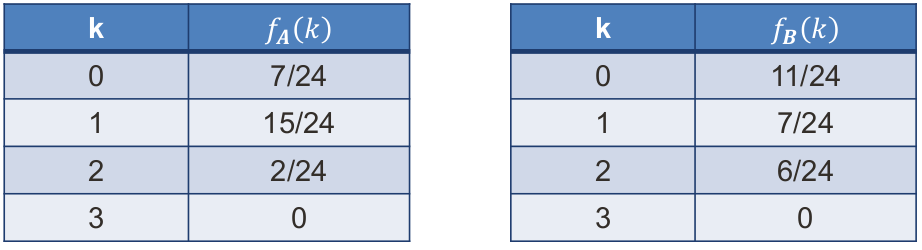
\includegraphics[width=0.6\textwidth]{figures/SimOptimiz_fi.png}
	\caption{Calculation of $f_i$ based on the example in
	\autoref{fig:SimOptimiz-ProcessLogic}}
\end{figure}

\subsubsection{FCFS prioritization rule}

What happens if we increase or decrease the items in stock $S_i$?

\begin{figure}[H]
	\centering
	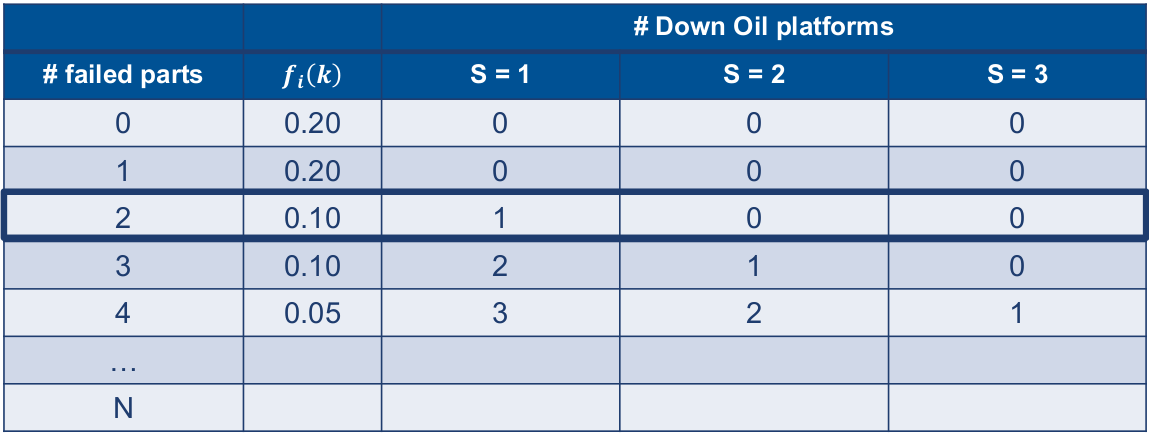
\includegraphics[width=0.65\textwidth]{figures/FCFSPrioritization.png}
	\caption{Number of down oil platforms based on different $S$}
\end{figure}

When we increase $S$ from 1 to 2, we will save during 10\% of time (namely
when number of defective parts equals 2) the downtime costs associated
with one oil platform. Also at days when the number of defective items for
the considered spare part is bigger than 3, we profit from reduced
downtime costs.

\paragraph{Optimization under FCFS}\mbox{}\\
\emph{Increase for each spare part the circulation stock as long as the
	marginal savings $[1-F(S)] b$ exceed the marginal (investment)
	$c_i$.}

\begin{equation}
S_i^* = min\{Q | F_i(Q) \ge \frac{b-c_i}{b}\}
\end{equation}

\subsubsection{Dynamic prioritization}

\begin{enumerate}
	\tightlist
	\item Spare parts causing downtime cost at this very moment, are prioritized
	over all other spare parts.
	\item If multiple spare parts are causing downtime cost, the one with the
	smallest average repair time will be selected (in order to get the next oil
	platform operational as soon as possible).
	\item When all oil platforms are running, we pick the spare part with the
	lowest "coverage".\\
	Coverage is here defined as: (current stock level +
	1) * average time between 2 subsequent failures.
\end{enumerate}

\emph{FCFS cannot be applied one-to-one!}

\paragraph{Optimization under dynamic prioritization}\mbox{}\\
In many (though not all) strong scheduling rules, repair priorities depend
on actual stock levels and thus on the circulation stock vector $S$. In
those cases, we cannot calculate optimal circulation stocks in one go as
in case of FCFS. An iterative heuristic can however do the job.

\paragraph{Iterative method for calculating $S^*$}

\begin{enumerate}
	\tightlist
	\item Develop (or use) an intelligent Prioritization rule $\Omega$.
	\item Initialize iteration count $n=0$ and circulation stock vector $S^n=0$.
	\item Simulate the system under $\Omega$ and $S^n$.\\
	Save the relative frequencies $i$, $f_i(k)$, $k\ge0$.
	\item Calculate $S^{n+1} = min\{Q|F_i(Q)\ge \frac{b-c_i}{b}\}$
	\item Stop when $S^{n+1} = S^n$. Otherwise $n = n+1$ and go to step 3.
\end{enumerate}